\section{Command Semantics}\label{sec:semantics}

We present the full semantics of atomic commands first,
then describe an important classification of expressions and substitutions,
before describing the semantics of the four composite command forms.

\subsection{Atomic Commands}\label{ssec:atomic}

The atomic command $\catom a$ can be very simply expressed as basic action
with the addition of healthiness conditions:
\RLEQNS{
   \lhsW &\defs& DL \land LE \land \WWW(P) & \elabel{\lblW}
\\ \lhsCA &\defs& \rhsCA & \elabel{\lblCA}
}
Here we would expect that if $LE$ holds when this action starts,
i.e. when $in \in ls$ and it gets to run,
that $LE'$ should also hold, with $out \in ls'$.

\subsection{Grounded and Sound}

Given that we have a distinction between static observations ($g$, $in$, $out$),
and dynamic ones ($s,s',ls,ls'$) it is worth extending this distinction
to expressions and substitutions.
The reason for this is do with the fact that, by design,
semantic sequantial composition ignores the static variables.
An expression or predicate is ``ground''
if the only variables present are static.
The $DL$ healthiness condition is ground,
but $LE$ is not, as it refers to $ls$.
Ground predicates $K$ satisfy some important laws:
\RLEQNS{
   K \seq K &=& K
\\ (K \land P)\seq Q &\;=\;& K \land (P\seq Q) \; = \; P \seq (K \land Q)
\\ K \land \WWW(P) &=& \WWW(K \land P)
} \noindent
A substitution is also deemed ``ground'',
if all the the replacement expressions are ground,
and the target variables are all static.
A desired consequence of this is that
ground substitutions $\gamma$
will distribute through semantic sequential composition,
semantic skip,
both disjoint label-set notations,
and $\WWW$
\RLEQNS{
   (P\seq Q)\gamma &=& P\gamma \seq Q\gamma  & \elabel{seq-gnd-distr}
\\ \Skip\gamma     &=& \Skip                 &\elabel{skip-gamma}
\\ ~\{L_1|\dots|L_n\}\gamma &=& \{L_1\gamma|\dots|L_n\gamma\}
& \elabel{DL-gamma-subst}
\\ ~[L_1|\dots|L_n]\gamma &=& [L_1\gamma|\dots|L_n\gamma]
& \elabel{LE-gamma-subst}
\\ (\WWW(P))\gamma &=& \WWW(P\gamma)
& \elabel{WwW-gamma-subst}
}
Groundness is not enough, we also require substitutions to be ``sound''
in the sense that they cannot transfrom a situation that satisfies $DL$
or $LE$ into one that does not.
A ground substitution $\varsigma$, of the form $[labs(G),I,O/g,in,out]$ is \emph{sound}
if $\setof{labs(G)|I|O}$ holds.
We will see that all substitutions in the semantic definitions
below are sound, and that this is easy to check by inspection.


\subsection{Composing Actions}\label{ssec:composing}

The semantics of composite actions basically involves using the generator
to produce a suitable number of labels,
that are then used in zero or more ``control-flow'' actions
of the form $A(E|ii|N)$, where $ii$ is atomic skip that simply asserts $s'=s$.
The left-over generator is the split as required,
and then the components are ``connected'' into
the relevant new labels and generators using sound substitutions.
Finally the relevant healthiness conditions are supplied.
A key principle is to ensure that when any sub-component is ``active'',
that is, at least one of its labels is present in $ls$,
that none of the labels of the parent,
other than those explicitly shared with the sub-component,
are themsleves in $ls$.
This prevents a parent starting a spurious copy of a sub-component
while that sub-component is actually running.
The semantic definitions are listed in Fig. \ref{fig:composite-semantics}.
Careful inspection of all the substitutions present will confirm that they
are all sound.
\begin{figure}[t]
  \RLEQNS{
     \lhsSEQ &\defs& \rhsSEQ & \elabel{\lblSEQ}
  \\ \lhsPAR
     &\defs&
     \leftW \rhsaPAR \lor {}
     & \elabel\lblPAR
  \\&& \phW \rhsbPAR \lor {}
  \\&& \phW \rhscPAR \lor {}
  \\&& \phW \rhsdPAR \rghtW
  \\ \lhsNDC &\defs& \rhsNDC & \elabel{\lblNDC}
  \\ \lhsSTAR
     &\defs&
     \leftW \rhsaSTAR \lor {}
     & \elabel\lblSTAR
  \\&& \phW \rhsbSTAR \lor {}
  \\&& \phW \rhscSTAR \lor {}
  \\&& \phW \rhsdSTAR \rghtW
  }
  \caption{Composite Semantics}
  \label{fig:composite-semantics}
\end{figure}

We will explain the semantics of parallel in more detail,
aided by the diagram in Fig. \ref{fig:PAR-plumbing}.
\begin{figure}
  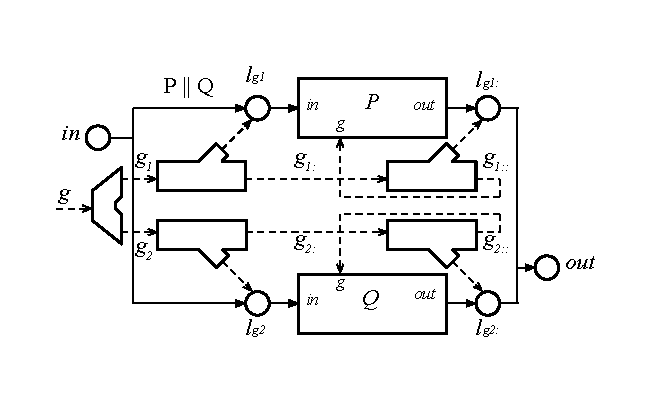
\includegraphics[scale=1.0]{images/PAR}
  \caption{Label and Generator ``plumbing'' for $P \parallel Q$.}
  \label{fig:PAR-plumbing}
\end{figure}
We take the generator $g$ and split it to obtain $\g1$ and $\g2$.
From $\g1$ we generate two labels $\ell_{g1}$ and $\ell_{g1:}$,
and leftover generator $\g{1::}$.
We then use a subtitution to replace all references
by $P$ to $g$, $in$ and $out$ with $\g{1::}$, $\ell_{g1}$ and $\ell_{g1:}$,
respectively. We do something similar with $\g2$ and $Q$.
We also add a top-level control action that is enabled by label $in$,
and adds both $\ell_{g1}$ and $\ell_{g2}$ into $ls$,
so enabling both $P$ and $Q$ to start.
We then have another control-flow action that waits for both of $\ell_{g1:}$
and $\ell_{g2:}$  to appear in $ls$,
at which point they will be replaced by the top-level $out$ label.

Given that the invariant $LE$, which is $[in|labs(g)|out]$,
is part of the definition of $\W$,
then we have it satisfied, by definition, by any sub-components.
From the perspective of the parent composite, this means that $LE\varsigma$
also holds, where $\varsigma$ ranges over all the sound substitutions
used in the definition of the parent's semantics.
For example, for program sequential composition,
we not only assert $[in|g|out]$,
but can also infer $[in|\g{:1}|\ell_g]$
and $[\ell_g|\g{:2}|out]$.


In summary,
we have have predicate semantics for atomic and composite program
constructs,
in which everything at every level is wrapped in an infinite loop.
This seems to be completely counter-intuitive:
a program that consists of a single atomic action may wait
for a while while external interference rumbles on,
but eventually it should get ``scheduled'', perform its atomic action
and then effectively stop.
How is this consistent with looping forever?
To see the answer to this question,
it helps to consider such simple examples,
and this brings up the issue of \emph{calculation}.
